\documentclass{jsarticle}
\usepackage{amsmath, bm} 
\usepackage[dvipdfmx]{graphicx}
\begin{document}

\title{統計データ解析課題1}
\author{J4-170273 奥田敬二郎}
\date{\today}
\maketitle

%================================================================
%     1
%================================================================
\section{}
$
\displaystyle \lim_{n \to \infty} I_n(f) = \int_{0}^{\infty} f(x) dx
$
なので、nを大きくすると計算結果は$\displaystyle \int_{0}^{\infty} f(x) dx$に近づく。

\subsection{}
$\displaystyle f(x) = \frac{1}{(1+x)^2}$
の時、
$\displaystyle \int_{0}^{\infty} f(x) dx = 1$
であり、計算結果は
\[
\left\{
	\begin{alignedat}{2}
		I_{10}(f) &= 0.8611662368776232\\
		I_{100}(f) &= 0.9851161663661924\\
		I_{1000}(f) &= 0.9985011661666946\\
		I_{10000}(f) &= 0.9998500116663119
	\end{alignedat}
\right.
\]

\subsection{}
$\displaystyle f(x) = \frac{2}{1+x^2}$
の時、
$\displaystyle \int_{0}^{\infty} f(x) dx = \pi$
であり、計算結果は
\[
\left\{
	\begin{alignedat}{2}
		I_{10}(f) &= 2.843242180027292\\
		I_{100}(f) &= 3.11159432008312\\
		I_{1000}(f) &= 3.1385926552561965\\
		I_{10000}(f) &= 3.141292653591556
	\end{alignedat}
\right.
\]

\subsection{ガウス積分}
$\displaystyle f(x) = \mathrm{exp}\left(-\frac{1}{2}x^2\right)$
の時、
$\displaystyle \int_{0}^{\infty} f(x) dx = \sqrt{\frac{\pi}{2}}$ , $\displaystyle \, 2 \left(\int_{0}^{\infty} f(x) dx\right)^2 = \pi$
であり、計算結果は

\[
\left\{
	\begin{alignedat}{2}
		I_{10}(f) &= 1.2033141373155003\\
		I_{100}(f) &= 1.2483141373155004\\
		I_{1000}(f) &= 1.25281413731549\\
		I_{10000}(f) &= 1.2532641373154276
	\end{alignedat}
\right.
\,\,\,\,
\left\{
	\begin{alignedat}{2}
		2 I_{10}(f)^2 &= 2.8959298261266935\\
		2 I_{100}(f)^2 &= 3.116576370843484\\
		2 I_{1000}(f)^2 &= 3.139086525315111\\
		2 I_{10000}(f)^2 &= 3.141341995761966
	\end{alignedat}
\right.
\]


\subsection{}
$
f(x) = 
  \left\{
    \begin{array}{ll}
      x^2 (1-x)^3 &(0<x<1)\\
      0 &(x\geq1)
    \end{array}
  \right.
$
の時、
$\displaystyle \int_{0}^{\infty} f(x) dx = \frac{1}{60}$
であり、計算結果は

\[
\left\{
	\begin{alignedat}{2}
		I_{10}(f) &= 0.016665000000000003\\
		I_{100}(f) &= 0.016666666499999993\\
		I_{1000}(f) &= 0.01666666666665003\\
		I_{10000}(f) &= 0.016666666666666576
	\end{alignedat}
\right.
\]
\\
%================================================================
%     2
%================================================================
\section{}
\subsection{}
$x_{j}\,(j=1,...,6) = 0.3835199,  1.3669469, -0.3452020,  1.3491541,  0.3029958,  0.5207242$\\
\[
  A	= \left(
    \begin{array}{cccc}
      0	         & 0.3835199  & 1.3669469  & -0.3452020\\
      -0.3835199 & 0          & 1.3491541  & 0.3029958\\
      -1.3669469 & -1.3491541 & 0          & 0.5207242\\
      0.3452020  & -0.3029958 & -0.5207242 & 0
    \end{array}
  \right)
\]
\[
  B	= \left(
    \begin{array}{cccc}
      0.24993987  & -0.4849698  & 0.8378762   & 0.01725761\\
      -0.71024416 & 0.27593963  & 0.360502    & 0.53800453\\
      -0.35887576 & -0.82909093 & -0.37703558 & 0.20410927\\
      0.55162622  & 0.03563492  & -0.16076676 & 0.81767519
    \end{array}
  \right)
\]

\subsection{}
\[\mathrm{detA} = 0.462674447965\, , \, \mathrm{detB} = 1\]

\subsection{}
固有値を$\lambda_{a_{i}}$、固有ベクトルを$\vec{a_{i}}\,\,(i = 1,2,3,4)$とすると
\begin{equation*}
\lambda_{a_{1}} = 8.32667268\cdot10^{-17}+2.05134642j, \,\,
\bm{a_{1}} = \left(
    \begin{alignedat}{1}
      -0.12411189 &- 0.4812949j\\
      0.12141420 &- 0.47230595j\\
      0.68536757 &+ 0.j\\
      -0.01123030 &+ 0.21279641j
    \end{alignedat}
  \right)
\end{equation*}
\begin{equation*}
\lambda_{a_{2}} = 8.32667268\cdot10^{-17}-2.05134642j, \,\,
\bm{a_{2}} = \left(
    \begin{alignedat}{1}
      -0.12411189&+0.4812949j\\
      0.12141420&+0.47230595j\\
      0.68536757&-0.j\\
      -0.01123030&-0.21279641j
    \end{alignedat}
  \right)
\end{equation*}
\begin{equation*}
\lambda_{a_{3}} = 4.16333634\cdot10^{-17}+0.33158796j, \,\,
\bm{a_{3}} = \left(
    \begin{alignedat}{1}
      0.14983522&+0.48010506j\\
      0.15108778&-0.48924244j\\
      0.01141575&+0.17361155j\\
      0.67423406&+0.j
    \end{alignedat}
  \right)
\end{equation*}
\begin{equation*}
\lambda_{a_{4}} = 4.16333634\cdot10^{-17}-0.33158796j, \,\,
\bm{a_{4}} = \left(
    \begin{alignedat}{1}
      0.14983522&-0.48010506j\\
      0.15108778&+0.48924244j\\
      0.01141575&-0.17361155j\\
      0.67423406&-0.j 
    \end{alignedat}
  \right)
\end{equation*}

\subsection{}
固有値を$\lambda_{b_{i}}$、固有ベクトルを$\vec{b_{i}}\,\,(i = 1,2,3,4)$とすると

\begin{equation*}
	\lambda_{b_{1}} = -0.46226703+0.88674077j, \,\,
		\bm{b_{1}} = \left(
		    \begin{alignedat}{1}
		      0.12411189&+0.4812949j\\
		      -0.12141420&+0.47230595j\\
		      -0.68536757&+0.j\\
		      0.01123030&-0.21279641j
		    \end{alignedat}
		  \right)
\end{equation*}

\begin{equation*}
	\lambda_{b_{2}} = -0.46226703-0.88674077j, \,\,
		\bm{b_{2}} = \left(
		    \begin{alignedat}{1}
		      0.12411189&-0.4812949j\\
		      -0.12141420&-0.47230595j\\
		      -0.68536757&-0.j\\
		      0.01123030&+0.21279641j
		    \end{alignedat}
		  \right)
\end{equation*}

\begin{equation*}
	\lambda_{b_{3}} = 0.94552658+0.3255449j, \,\,
		\bm{b_{3}} = \left(
		    \begin{alignedat}{1}
		      0.14983522&+0.48010506j\\
		      0.15108778&-0.48924244j\\
		      0.01141575&+0.17361155j\\
		      0.67423406&+0.j
		    \end{alignedat}
		  \right)
\end{equation*}

\begin{equation*}
	\lambda_{b_{4}} = 0.94552658-0.3255449j, \,\,
		\bm{b_{4}} = \left(
		    \begin{alignedat}{1}
		      0.14983522&-0.48010506j\\
		      0.15108778&+0.48924244j\\
		      0.01141575&-0.17361155j\\
		      0.67423406&-0.j 
		    \end{alignedat}
		  \right)
\end{equation*}

\subsection{}
$A$の固有値の指数関数は
\[
\left\{
	\begin{alignedat}{1}
		-0.4622670324619393&+0.8867407686008535j\\
		-0.4622670324619393&-0.8867407686008535j\\
		0.945526584150717&+0.3255448950057075j\\
		0.945526584150717&-0.3255448950057075j
	\end{alignedat}
\right.
\]
これらは$B$の固有値とほとんど等しい\\
また、上記の2.3、2.4から分かるように、$A$と$B$の固有ベクトルもほとんど等しい\\
さらに、$\displaystyle B = I_{4} + \sum_{n=1}^{m} \frac{1}{n!} A^{n}$として、$A$の固有値の指数関数と、$B$の固有値の値の差の絶対値の和$d\,\,$($\displaystyle = \sum_{i=1}^{4} |\mathrm{exp}(\lambda_{a_{i}}) - \lambda_{b_{i}}|$)
として、横軸$m$、縦軸$d$のグラフにすると、\\
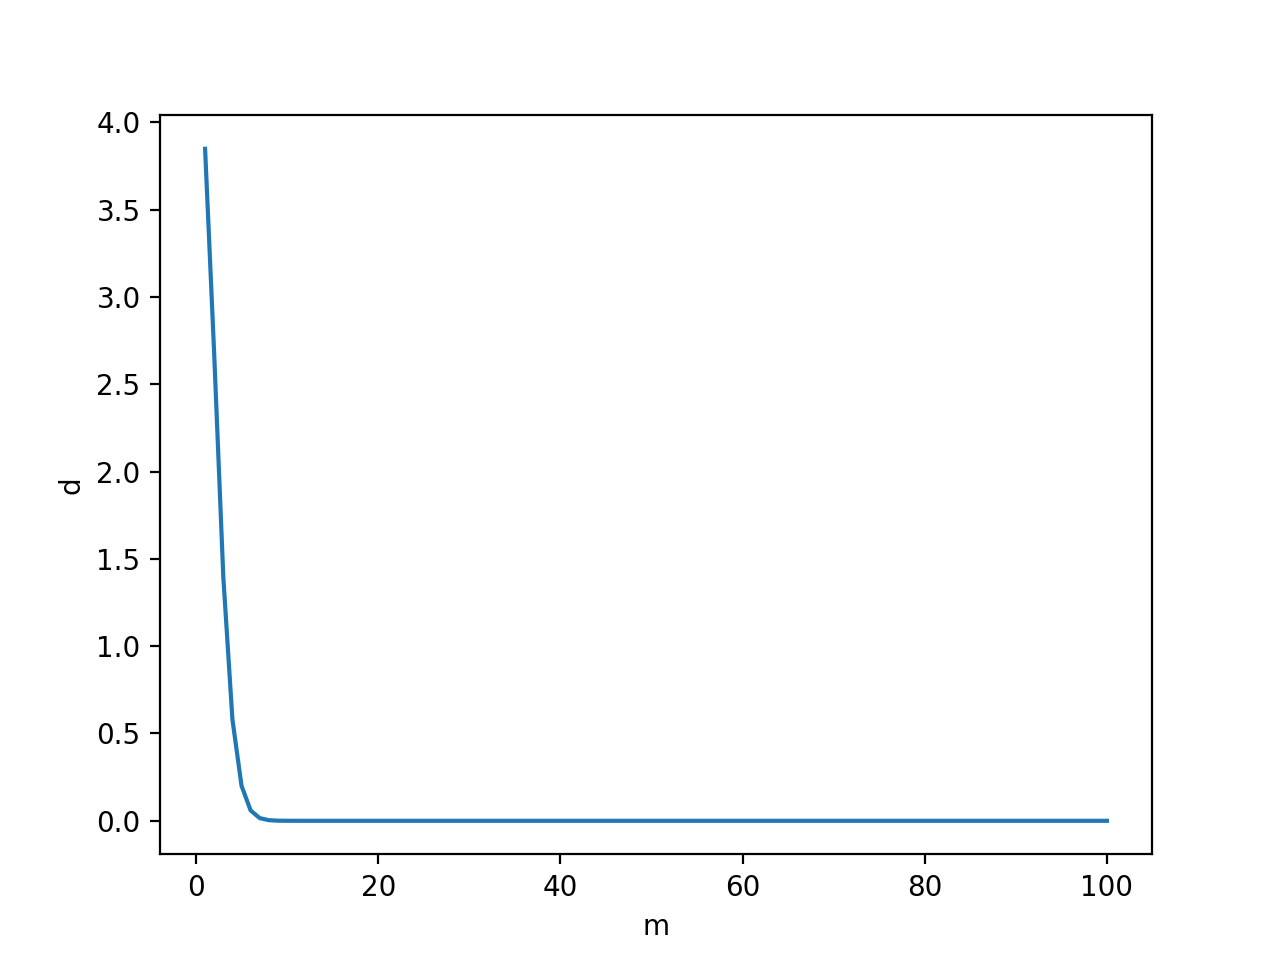
\includegraphics{1.png}\\
となり、$m$が大きくなると$B$の固有値は$A$の固有値の指数関数に収束すると推測される。
\\
%================================================================
%     3
%================================================================
\section{}
t分布の確率密度関数は、
$\displaystyle f(t) = \frac{\Gamma((\nu+1)/2)}{\sqrt{\nu\pi}\,\Gamma(\nu)} (1+t^{2}/\nu)^{-(\nu+1)/2}$\,\,
($\nu$は自由度、$\Gamma$はガンマ関数)であり、
$\displaystyle \lim_{\nu \to \infty} f(x) = \frac{1}{\sqrt{2\pi}\sigma} \, \mathrm{exp} \left( -\frac{x^{2}}{2\sigma^{2}} \right) = $
”$N(0,\sigma^2)$の確率密度関数”(ただし$\sigma^2 = (1-\theta^2)^{-1}$)となる

\subsection{}
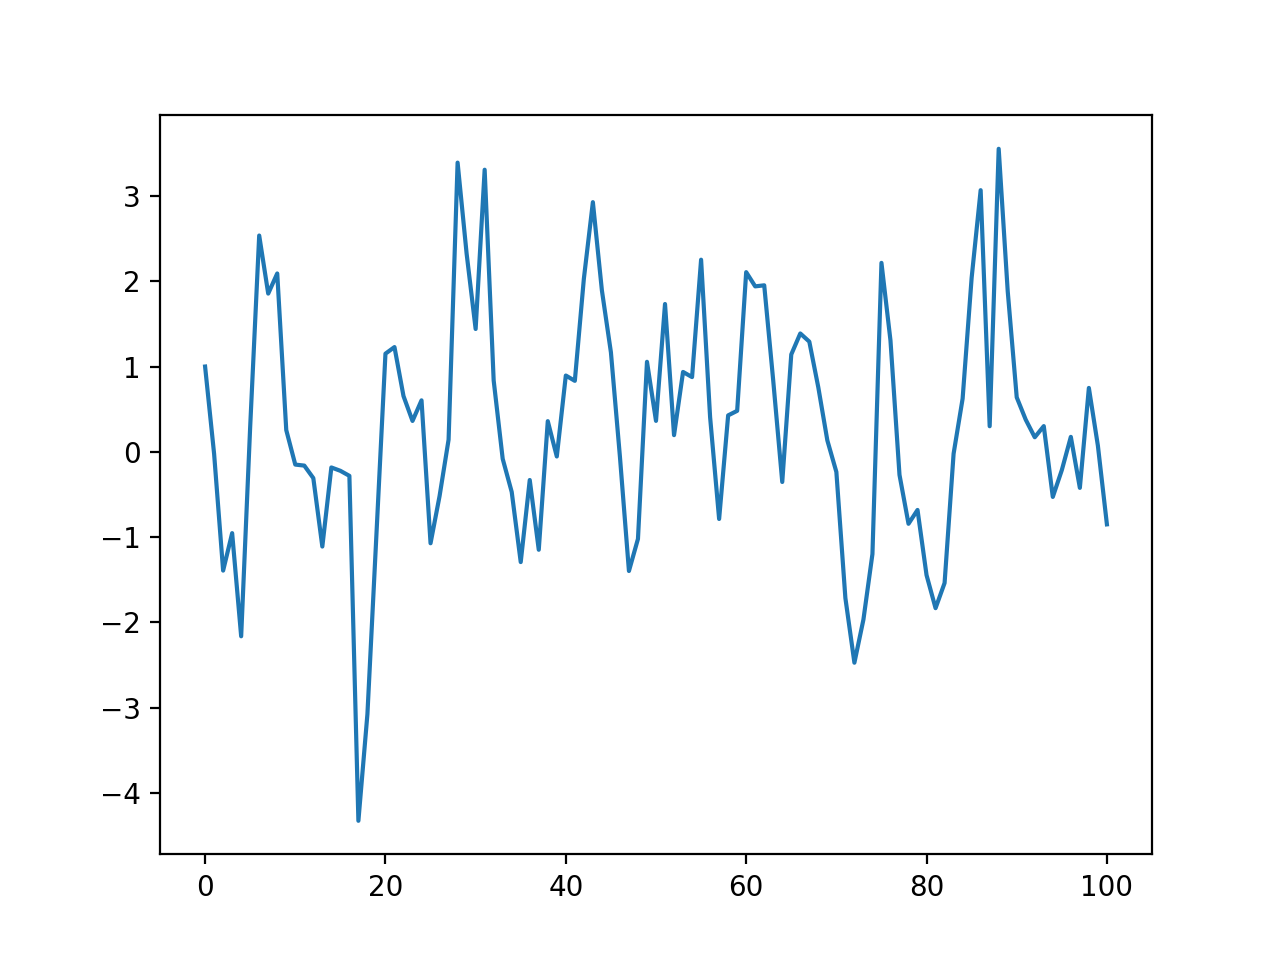
\includegraphics{2.png}

\subsection{}
$T=10^5$の時
\[
(T+1)^{-1} \sum_{t=0}^{T} X_{t} = -0.00371338716465, \,\, T^{-1}\sum_{t=1}^{T} X_{t-1}^2 = 1.96217931557
\]
\subsection{}
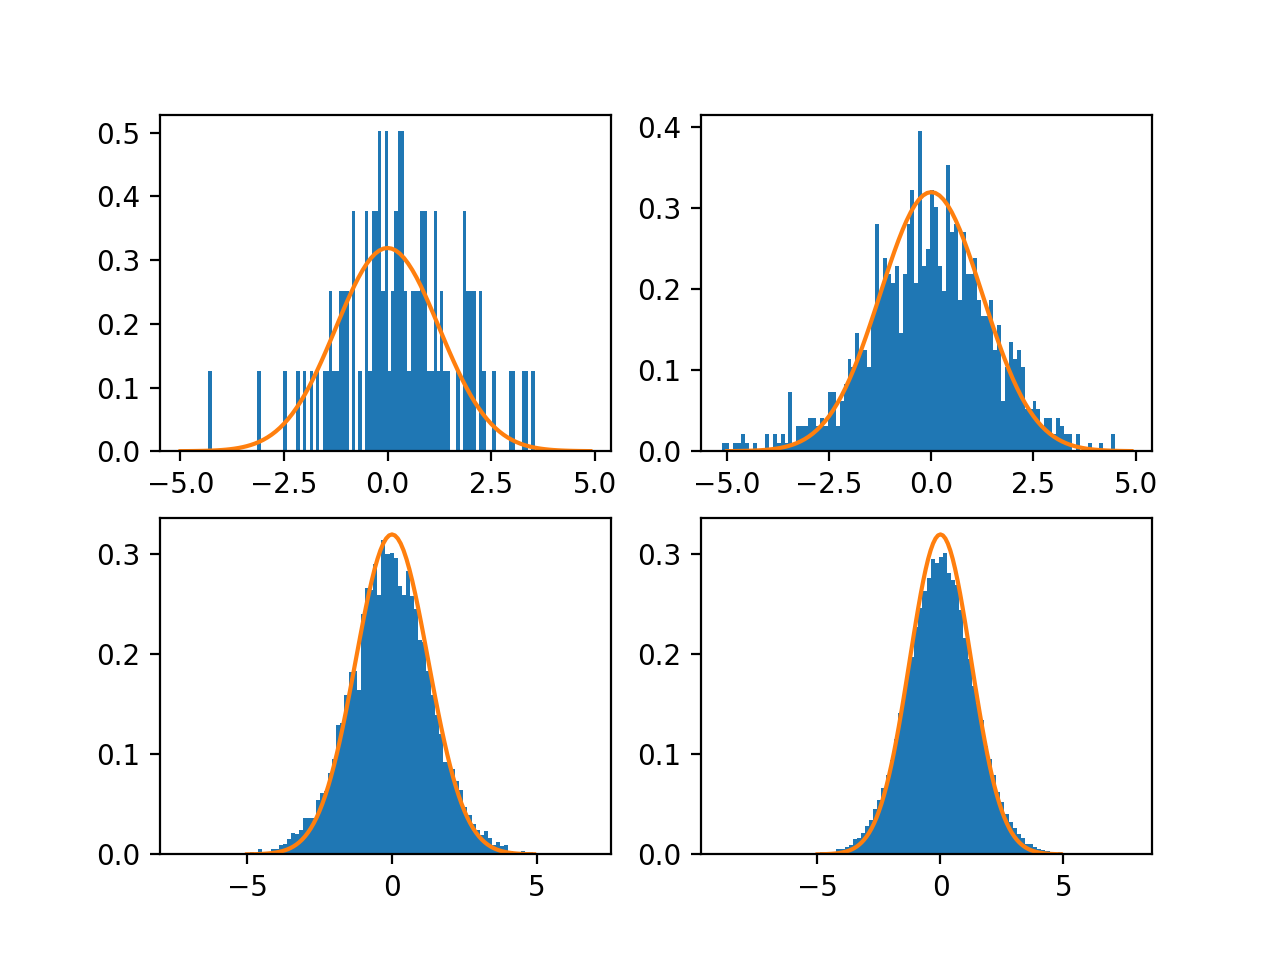
\includegraphics{3.png}
また、自由度$\nu$を$100000$と大きくしてみると、$T^{-1}\sum_{t=1}^{T} X_{t-1}^2 = 1.55918524828$となり、
これは$\sigma^2 = (1-\theta^2)^{-1} = 1.5625$に近い値になる。その時のヒストグラムは以下のようになり、確かに$\nu$が$\infty$に近づくことで正規分布に近づくことが確認できる。\\
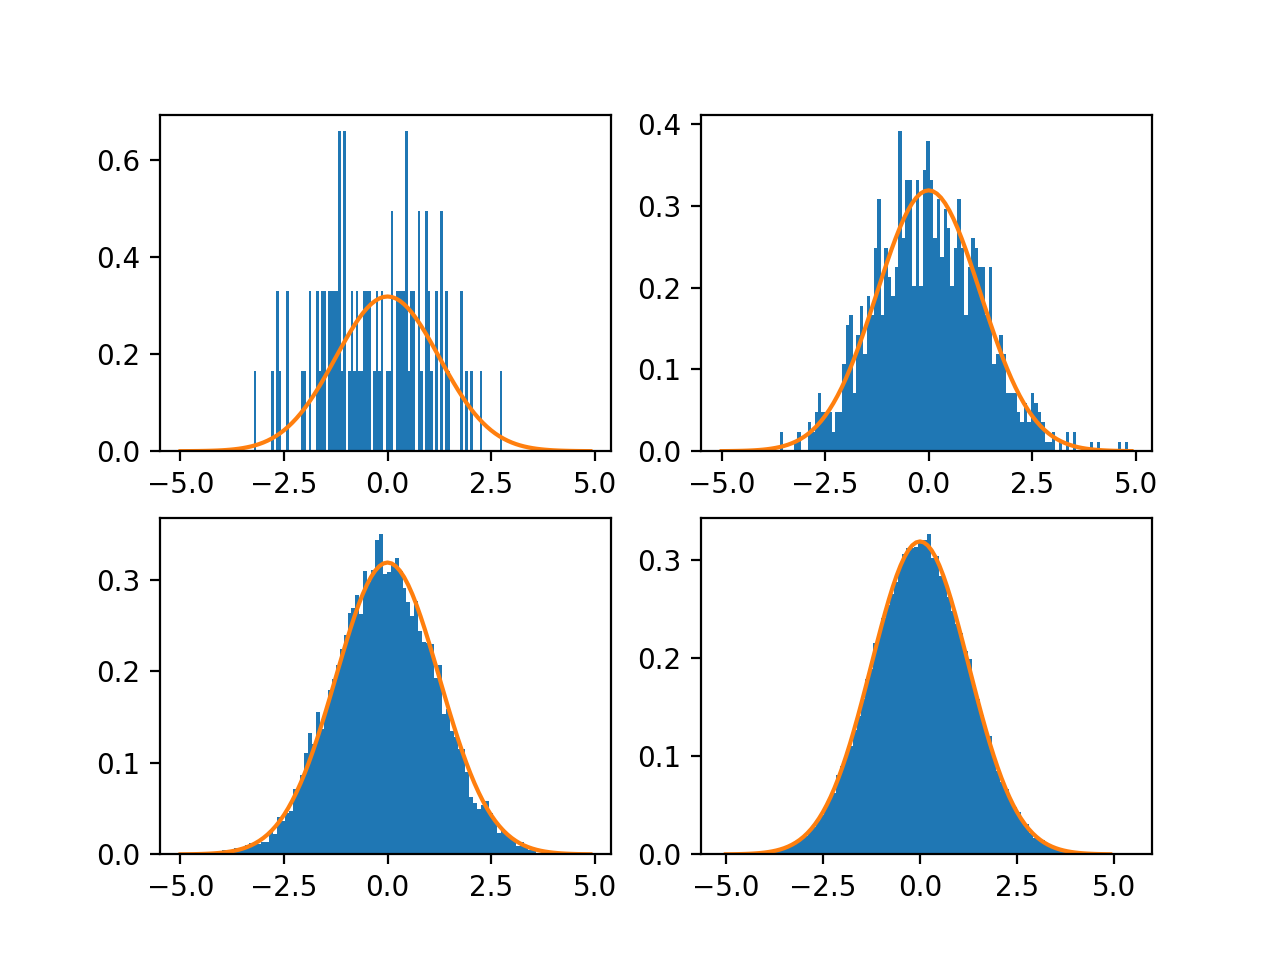
\includegraphics{4.png}

%================================================================
%     4
%================================================================
\section{ウィグナー行列}
\subsection{}
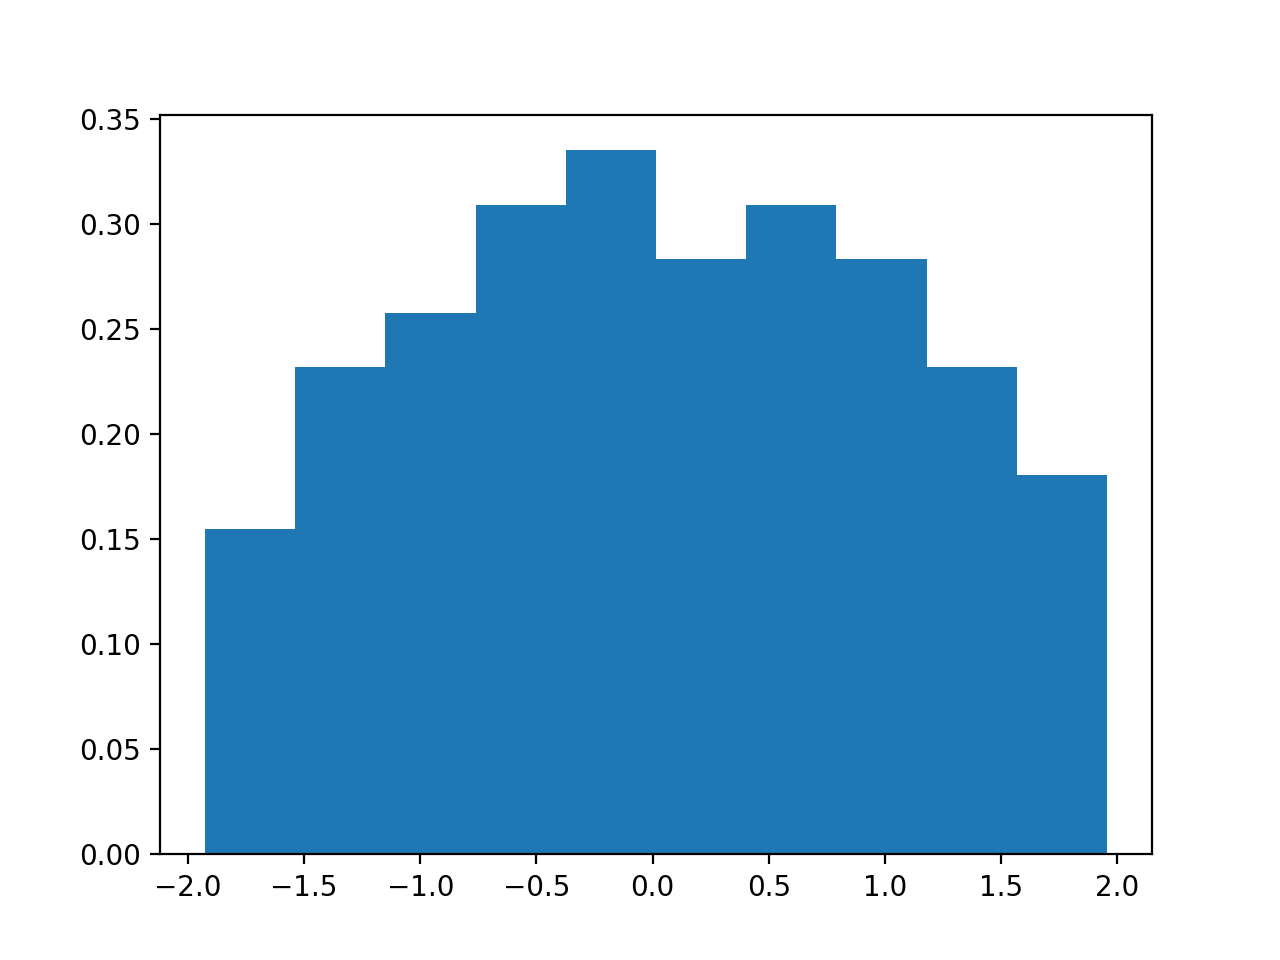
\includegraphics{5.png}

\subsection{ウィグナーの半円則}
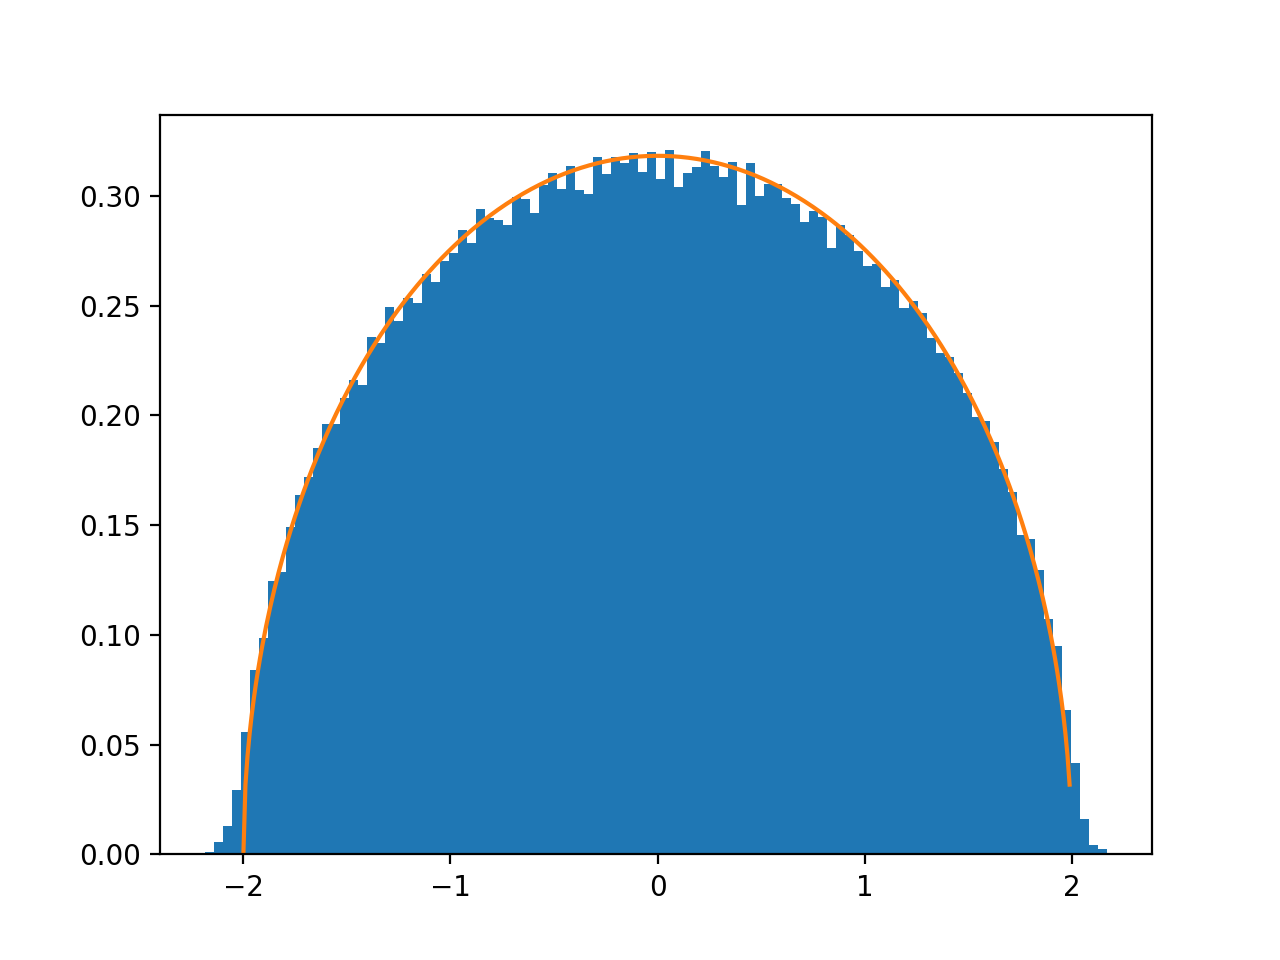
\includegraphics{6.png}
\\
ランダム行列を10000個生成すると以下のようになり、より楕円にフィットする。
\\
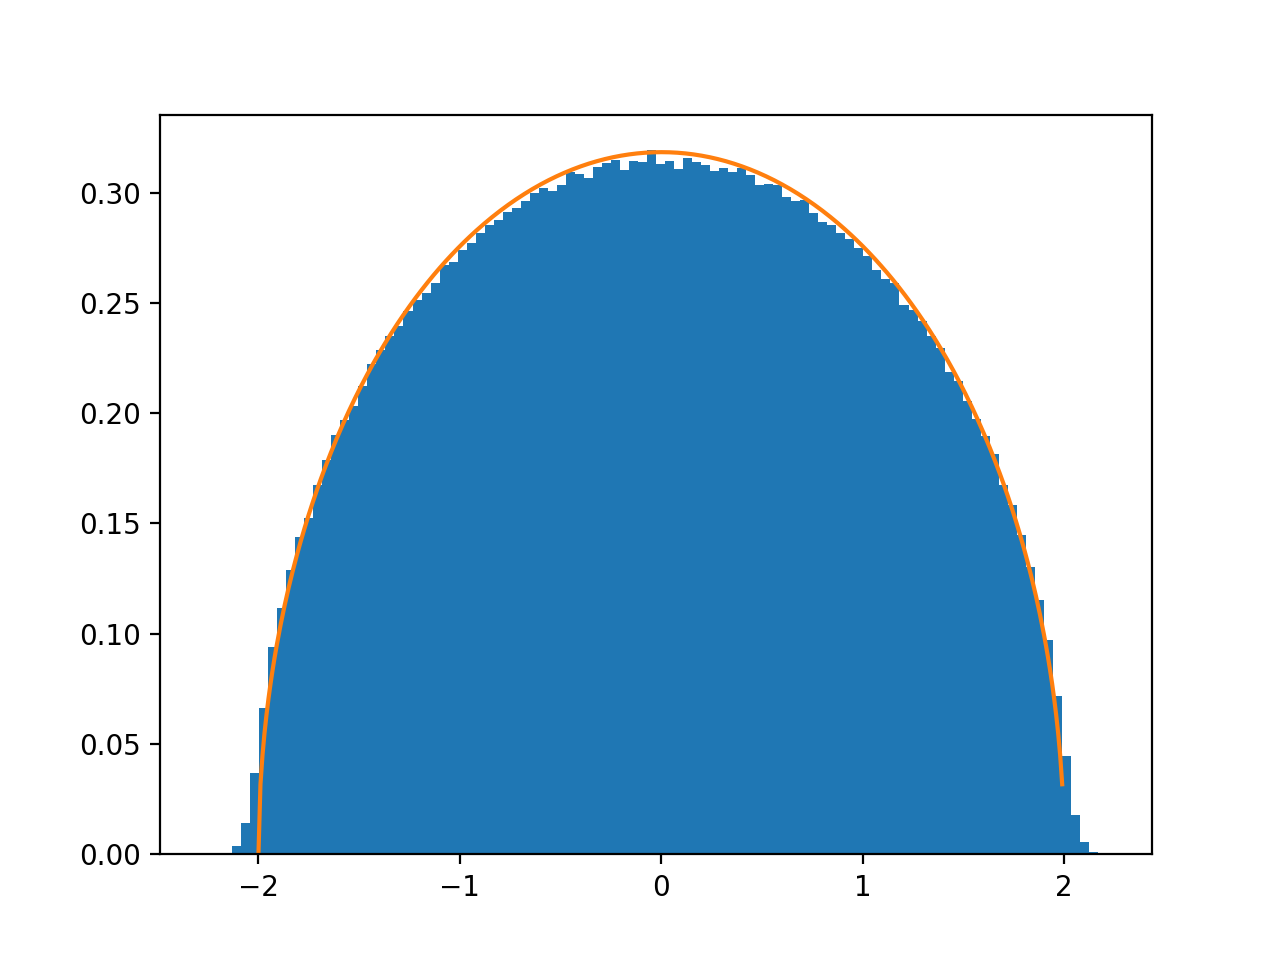
\includegraphics{7.png}



















\end{document}